% Options for packages loaded elsewhere
\PassOptionsToPackage{unicode}{hyperref}
\PassOptionsToPackage{hyphens}{url}
\PassOptionsToPackage{dvipsnames,svgnames,x11names}{xcolor}
%
\documentclass[
  a4paper,
]{article}

\usepackage{amsmath,amssymb}
\usepackage{iftex}
\ifPDFTeX
  \usepackage[T1]{fontenc}
  \usepackage[utf8]{inputenc}
  \usepackage{textcomp} % provide euro and other symbols
\else % if luatex or xetex
  \usepackage{unicode-math}
  \defaultfontfeatures{Scale=MatchLowercase}
  \defaultfontfeatures[\rmfamily]{Ligatures=TeX,Scale=1}
\fi
\usepackage{lmodern}
\ifPDFTeX\else  
    % xetex/luatex font selection
\fi
% Use upquote if available, for straight quotes in verbatim environments
\IfFileExists{upquote.sty}{\usepackage{upquote}}{}
\IfFileExists{microtype.sty}{% use microtype if available
  \usepackage[]{microtype}
  \UseMicrotypeSet[protrusion]{basicmath} % disable protrusion for tt fonts
}{}
\makeatletter
\@ifundefined{KOMAClassName}{% if non-KOMA class
  \IfFileExists{parskip.sty}{%
    \usepackage{parskip}
  }{% else
    \setlength{\parindent}{0pt}
    \setlength{\parskip}{6pt plus 2pt minus 1pt}}
}{% if KOMA class
  \KOMAoptions{parskip=half}}
\makeatother
\usepackage{xcolor}
\usepackage[top=2.54cm,right=2.54cm,bottom=2.54cm,left=2.54cm]{geometry}
\setlength{\emergencystretch}{3em} % prevent overfull lines
\setcounter{secnumdepth}{-\maxdimen} % remove section numbering
% Make \paragraph and \subparagraph free-standing
\ifx\paragraph\undefined\else
  \let\oldparagraph\paragraph
  \renewcommand{\paragraph}[1]{\oldparagraph{#1}\mbox{}}
\fi
\ifx\subparagraph\undefined\else
  \let\oldsubparagraph\subparagraph
  \renewcommand{\subparagraph}[1]{\oldsubparagraph{#1}\mbox{}}
\fi


\providecommand{\tightlist}{%
  \setlength{\itemsep}{0pt}\setlength{\parskip}{0pt}}\usepackage{longtable,booktabs,array}
\usepackage{calc} % for calculating minipage widths
% Correct order of tables after \paragraph or \subparagraph
\usepackage{etoolbox}
\makeatletter
\patchcmd\longtable{\par}{\if@noskipsec\mbox{}\fi\par}{}{}
\makeatother
% Allow footnotes in longtable head/foot
\IfFileExists{footnotehyper.sty}{\usepackage{footnotehyper}}{\usepackage{footnote}}
\makesavenoteenv{longtable}
\usepackage{graphicx}
\makeatletter
\def\maxwidth{\ifdim\Gin@nat@width>\linewidth\linewidth\else\Gin@nat@width\fi}
\def\maxheight{\ifdim\Gin@nat@height>\textheight\textheight\else\Gin@nat@height\fi}
\makeatother
% Scale images if necessary, so that they will not overflow the page
% margins by default, and it is still possible to overwrite the defaults
% using explicit options in \includegraphics[width, height, ...]{}
\setkeys{Gin}{width=\maxwidth,height=\maxheight,keepaspectratio}
% Set default figure placement to htbp
\makeatletter
\def\fps@figure{htbp}
\makeatother

% Preámbulo
\usepackage{comment} % Permite comentar secciones del código
\usepackage{marvosym} % Agrega símbolos adicionales
\usepackage{graphicx} % Permite insertar imágenes
\usepackage{mathptmx} % Fuente de texto matemática
\usepackage{amssymb} % Símbolos adicionales de matemáticas
\usepackage{lipsum} % Crea texto aleatorio
\usepackage{amsthm} % Teoremas y entornos de demostración
\usepackage{float} % Control de posiciones de figuras y tablas
\usepackage{rotating} % Rotación de elementos
\usepackage{multirow} % Celdas combinadas en tablas
\usepackage{tabularx} % Tablas con ancho de columna ajustable
\usepackage{mdframed} % Marcos alrededor de elementos flotantes

% Series de tiempo
\usepackage{booktabs}


% Configuración adicional

\makeatletter
\makeatother
\makeatletter
\makeatother
\makeatletter
\@ifpackageloaded{caption}{}{\usepackage{caption}}
\AtBeginDocument{%
\ifdefined\contentsname
  \renewcommand*\contentsname{Tabla de contenidos}
\else
  \newcommand\contentsname{Tabla de contenidos}
\fi
\ifdefined\listfigurename
  \renewcommand*\listfigurename{Listado de Figuras}
\else
  \newcommand\listfigurename{Listado de Figuras}
\fi
\ifdefined\listtablename
  \renewcommand*\listtablename{Listado de Tablas}
\else
  \newcommand\listtablename{Listado de Tablas}
\fi
\ifdefined\figurename
  \renewcommand*\figurename{Figura}
\else
  \newcommand\figurename{Figura}
\fi
\ifdefined\tablename
  \renewcommand*\tablename{Tabla}
\else
  \newcommand\tablename{Tabla}
\fi
}
\@ifpackageloaded{float}{}{\usepackage{float}}
\floatstyle{ruled}
\@ifundefined{c@chapter}{\newfloat{codelisting}{h}{lop}}{\newfloat{codelisting}{h}{lop}[chapter]}
\floatname{codelisting}{Listado}
\newcommand*\listoflistings{\listof{codelisting}{Listado de Listados}}
\makeatother
\makeatletter
\@ifpackageloaded{caption}{}{\usepackage{caption}}
\@ifpackageloaded{subcaption}{}{\usepackage{subcaption}}
\makeatother
\makeatletter
\@ifpackageloaded{tcolorbox}{}{\usepackage[skins,breakable]{tcolorbox}}
\makeatother
\makeatletter
\@ifundefined{shadecolor}{\definecolor{shadecolor}{rgb}{.97, .97, .97}}
\makeatother
\makeatletter
\makeatother
\makeatletter
\makeatother
\ifLuaTeX
\usepackage[bidi=basic]{babel}
\else
\usepackage[bidi=default]{babel}
\fi
\babelprovide[main,import]{spanish}
% get rid of language-specific shorthands (see #6817):
\let\LanguageShortHands\languageshorthands
\def\languageshorthands#1{}
\ifLuaTeX
  \usepackage{selnolig}  % disable illegal ligatures
\fi
\usepackage[]{biblatex}
\addbibresource{../../../../references.bib}
\IfFileExists{bookmark.sty}{\usepackage{bookmark}}{\usepackage{hyperref}}
\IfFileExists{xurl.sty}{\usepackage{xurl}}{} % add URL line breaks if available
\urlstyle{same} % disable monospaced font for URLs
\hypersetup{
  pdftitle={Perspectivas Globales. Explorando los Fundamentos y Alcances de las Finanzas Internacionales},
  pdfauthor={Edison Achalma},
  pdflang={es},
  colorlinks=true,
  linkcolor={blue},
  filecolor={Maroon},
  citecolor={Blue},
  urlcolor={Blue},
  pdfcreator={LaTeX via pandoc}}

\title{Perspectivas Globales. Explorando los Fundamentos y Alcances de
las Finanzas Internacionales}
\usepackage{etoolbox}
\makeatletter
\providecommand{\subtitle}[1]{% add subtitle to \maketitle
  \apptocmd{\@title}{\par {\large #1 \par}}{}{}
}
\makeatother
\subtitle{Un análisis en profundidad de los conceptos clave y su
relevancia en un mundo interconectado}
\author{Edison Achalma}
\date{2023-06-16}

\begin{document}
\maketitle
\ifdefined\Shaded\renewenvironment{Shaded}{\begin{tcolorbox}[enhanced, interior hidden, boxrule=0pt, borderline west={3pt}{0pt}{shadecolor}, sharp corners, frame hidden, breakable]}{\end{tcolorbox}}\fi

\hypertarget{oruxedgenes-y-conceptos-fundamentales-de-las-finanzas-internacionales}{%
\section{Orígenes y Conceptos Fundamentales de las Finanzas
Internacionales}\label{oruxedgenes-y-conceptos-fundamentales-de-las-finanzas-internacionales}}

\hypertarget{economuxeda-internacional}{%
\subsection{Economía Internacional}\label{economuxeda-internacional}}

El campo de las finanzas internacionales es de vital importancia en el
ámbito económico global, ya que abarca una amplia gama de temas
relacionados con las transacciones financieras entre países y el
funcionamiento de los mercados financieros internacionales. A
continuación, se exploran los conceptos clave que sustentan las finanzas
internacionales.

\begin{enumerate}
\def\labelenumi{\arabic{enumi}.}
\item
  \textbf{Regímenes Cambiarios:} Los regímenes cambiarios se refieren al
  conjunto de políticas y acuerdos que determinan cómo se fijan los
  tipos de cambio entre las distintas monedas. Existen diferentes tipos
  de regímenes cambiarios, como tipos de cambio fijos, flexibles o
  ajustables, y cada uno tiene implicaciones en la estabilidad monetaria
  y en las transacciones internacionales.
\item
  \textbf{Sistema Monetario Internacional:} El sistema monetario
  internacional comprende las instituciones, acuerdos y mecanismos que
  regulan las transacciones financieras y el intercambio de monedas
  entre países. Este sistema facilita el comercio internacional y la
  inversión al establecer reglas y procedimientos para el intercambio de
  divisas, los pagos internacionales y la gestión de las reservas
  internacionales.
\item
  \textbf{Procesos de Ajuste en la Balanza de Pagos:} La balanza de
  pagos registra todas las transacciones económicas y financieras entre
  un país y el resto del mundo. Los procesos de ajuste se refieren a los
  mecanismos mediante los cuales los países corrigen los desequilibrios
  en sus balanzas de pagos, como los déficits o los superávits. Estos
  ajustes pueden implicar cambios en los tipos de cambio, políticas
  monetarias o fiscales, y afectan la competitividad y la estabilidad
  económica de los países.
\item
  \textbf{Determinantes del Tipo de Cambio:} El tipo de cambio es el
  precio relativo entre dos monedas y juega un papel crucial en las
  transacciones internacionales. Los factores que influyen en el tipo de
  cambio incluyen los diferenciales de tasas de interés, la inflación,
  los flujos de capital, la política económica y las expectativas del
  mercado. Comprender estos determinantes es fundamental para analizar
  los movimientos y la volatilidad de las divisas.
\item
  \textbf{Condiciones de Paridad:} Las condiciones de paridad son
  teorías que establecen relaciones entre los tipos de cambio y los
  precios relativos en diferentes países. Estas teorías incluyen la
  paridad de tasas de interés, que establece una relación entre las
  tasas de interés y los tipos de cambio, y la paridad de poder
  adquisitivo, que establece una relación entre los niveles de precios y
  los tipos de cambio. Estas condiciones proporcionan un marco teórico
  para entender las interacciones entre las variables económicas y los
  tipos de cambio.
\end{enumerate}

\hypertarget{finanzas-corporativas}{%
\subsection{Finanzas Corporativas}\label{finanzas-corporativas}}

En el ámbito de las finanzas corporativas, las empresas se enfrentan a
desafíos y oportunidades en el contexto de un entorno global. Los
conceptos clave en finanzas corporativas internacionales son los
siguientes:

\begin{enumerate}
\def\labelenumi{\arabic{enumi}.}
\item
  \textbf{Mercados Financieros Internacionales:} Los mercados
  financieros internacionales son aquellos en los que se negocian
  activos financieros, como acciones, bonos, divisas y derivados, entre
  inversores de diferentes países. Estos mercados proporcionan a las
  empresas acceso a fuentes de financiamiento globales, permitiéndoles
  captar capital y gestionar los riesgos asociados a las fluctuaciones
  de los tipos de cambio y las tasas de interés.
\item
  \textbf{Operaciones a Escala Mundial:} Las empresas internacionales
  realizan operaciones comerciales y financieras en múltiples países, lo
  que implica la gestión de aspectos como el comercio internacional, la
  inversión extranjera directa y las alianzas estratégicas. Estas
  operaciones requieren una comprensión profunda de las diferencias en
  las regulaciones, los sistemas fiscales, los riesgos políticos y los
  aspectos culturales de cada país.
\item
  \textbf{Evaluación y Gestión del Riesgo Cambiario:} El riesgo
  cambiario se refiere a las pérdidas potenciales que una empresa puede
  sufrir debido a las fluctuaciones adversas en los tipos de cambio. La
  evaluación y gestión del riesgo cambiario involucra la identificación,
  medición y aplicación de estrategias para mitigar el impacto de las
  fluctuaciones cambiarias en los resultados financieros de la empresa.
  Estas estrategias pueden incluir el uso de instrumentos derivados,
  como los contratos de futuros o las opciones, para cubrir las
  exposiciones al riesgo cambiario.
\item
  \textbf{Financiamiento Internacional:} El financiamiento internacional
  se refiere a la obtención de capital por parte de las empresas en los
  mercados financieros internacionales. Esto puede incluir la emisión de
  bonos en mercados extranjeros, la obtención de préstamos de bancos
  internacionales o el acceso a inversionistas globales a través de la
  emisión de acciones en los mercados de valores internacionales. El
  financiamiento internacional proporciona a las empresas los recursos
  necesarios para financiar sus operaciones y proyectos a nivel mundial.
\item
  \textbf{Inversión en Portafolios Internacionales:} La inversión en
  portafolios internacionales implica la adquisición de activos
  financieros, como acciones y bonos, emitidos por empresas o gobiernos
  extranjeros. Los inversores internacionales diversifican sus carteras
  de inversión para aprovechar las oportunidades de rendimiento y
  reducir los riesgos asociados con la concentración en un solo país o
  una sola moneda. La inversión en portafolios internacionales requiere
  un análisis detallado de los mercados financieros y una evaluación de
  los riesgos y las oportunidades en cada país.
\end{enumerate}

Al comprender estos conceptos en los campos de la economía internacional
y las finanzas corporativas, se puede tener una visión más completa de
los aspectos fundamentales que sustentan las transacciones financieras
internacionales y las operaciones corporativas en un entorno global en
constante cambio.

\begin{figure}[H]

{\centering 
\includegraphics[width=5.5in,height=3.5in]{index_files/figure-latex/dot-figure-1.png}

}

\end{figure}

\hypertarget{finanzas-internacionales-conceptos-y-relevancia}{%
\section{Finanzas Internacionales: Conceptos y
Relevancia}\label{finanzas-internacionales-conceptos-y-relevancia}}

\hypertarget{quuxe9-son-las-finanzas-internacionales}{%
\subsection{¿Qué son las Finanzas
Internacionales?}\label{quuxe9-son-las-finanzas-internacionales}}

Las finanzas internacionales constituyen un campo de estudio que se
enfoca en analizar los flujos de efectivo y la valuación de activos en
un contexto global. Este ámbito abarca tanto los movimientos de capital
entre países como la valoración de activos ubicados en diferentes
naciones y denominados en diversas monedas. Las finanzas internacionales
son fundamentales para comprender y gestionar las transacciones
financieras que trascienden las fronteras nacionales.

\hypertarget{administraciuxf3n-financiera-internacional}{%
\subsection{Administración Financiera
Internacional}\label{administraciuxf3n-financiera-internacional}}

La administración financiera internacional se refiere al proceso de toma
de decisiones financieras por parte de ejecutivos de empresas
multinacionales que operan en un entorno global. Estas decisiones están
influenciadas por una serie de factores, como los riesgos asociados a
los flujos de efectivo a través de distintos marcos políticos y legales,
así como la exposición a fluctuaciones en los tipos de cambio. La
administración financiera internacional implica considerar tanto los
aspectos económicos como los monetarios de la economía global.

\hypertarget{importancia-del-riesgo-poluxedtico-y-de-tipo-de-cambio}{%
\subsection{Importancia del Riesgo Político y de Tipo de
Cambio}\label{importancia-del-riesgo-poluxedtico-y-de-tipo-de-cambio}}

En el ámbito de las finanzas internacionales, es crucial tener en cuenta
los riesgos asociados a los flujos de efectivo en diferentes países y
monedas. El riesgo político se refiere a la incertidumbre y las posibles
consecuencias que surgen de los cambios en los marcos políticos y
legales de un país. Por otro lado, el riesgo de tipo de cambio se
relaciona con la volatilidad en las tasas de cambio entre distintas
monedas. Estos riesgos pueden afectar significativamente los resultados
financieros de las organizaciones y deben ser gestionados adecuadamente.

\hypertarget{imperfecciones-de-los-mercados-internacionales}{%
\subsection{Imperfecciones de los Mercados
Internacionales}\label{imperfecciones-de-los-mercados-internacionales}}

Los mercados financieros internacionales presentan diversas
imperfecciones que pueden generar tanto amenazas como oportunidades para
las organizaciones. Entre estas imperfecciones se encuentran los costos
de transacción, los costos de información, las restricciones legales,
las diferencias en los sistemas impositivos, la movilidad imperfecta de
los factores de producción y las obstrucciones al comercio, entre otros.
Comprender y manejar estas imperfecciones es esencial para aprovechar
las oportunidades y mitigar los riesgos asociados a las operaciones
internacionales.

\hypertarget{generaciuxf3n-de-valor-y-problema-de-agencia}{%
\subsection{Generación de Valor y Problema de
Agencia}\label{generaciuxf3n-de-valor-y-problema-de-agencia}}

El objetivo principal en las finanzas internacionales es generar valor
para las empresas. La fórmula utilizada para medir este valor es la
siguiente:

\[
Valor = \sum_{t=1}^{n} \frac{E(FE_t)}{(1+k)^t}
\]

Donde \(E(FE_t)\) representa los flujos de efectivo esperados en el
periodo t, k es la tasa de descuento y n es el número total de periodos
considerados. Sin embargo, en un entorno financiero cada vez más
integrado e interdependiente, surge el problema de agencia, que implica
conflictos de intereses entre los diferentes participantes del mercado y
los ejecutivos de las organizaciones. Este problema debe ser abordado de
manera efectiva para garantizar la maximización del valor para los
accionistas y la sostenibilidad de las empresas en el largo plazo.

\hypertarget{globalizaciuxf3n-un-nuevo-paradigma-econuxf3mico}{%
\subsection{Globalización: Un Nuevo Paradigma
Económico}\label{globalizaciuxf3n-un-nuevo-paradigma-econuxf3mico}}

\hypertarget{la-globalizaciuxf3n}{%
\subsubsection{La Globalización}\label{la-globalizaciuxf3n}}

La globalización es un proceso de integración económica, social y
política que tiene como objetivo la creación de un mercado mundial
unificado. En este mercado, se comercian productos similares, producidos
por empresas cuyas operaciones se extienden a varios países, lo que
dificulta determinar su origen exacto. La globalización no solo se
manifiesta en el ámbito de la producción, sino también en la inversión y
el consumo.

\hypertarget{la-globalizaciuxf3n-en-distintas-uxe1reas}{%
\subsubsection{La Globalización en Distintas
Áreas}\label{la-globalizaciuxf3n-en-distintas-uxe1reas}}

El proceso de globalización no se desarrolla de manera uniforme en todas
las áreas. Algunas regiones están más avanzadas en términos de
integración económica global que otras. Por ejemplo, el mercado de
divisas se ha vuelto más integrado, con la existencia de un precio único
para las diferentes monedas. Asimismo, los mercados de capital están
experimentando un rápido avance en su integración, facilitando la
movilidad de los flujos financieros a nivel mundial.

\hypertarget{factores-que-impulsan-la-globalizaciuxf3n}{%
\subsubsection{Factores que Impulsan la
Globalización}\label{factores-que-impulsan-la-globalizaciuxf3n}}

La creciente globalización se ha visto influenciada por diversos
factores. Algunos de los principales son:

\begin{enumerate}
\def\labelenumi{\arabic{enumi}.}
\item
  \textbf{Reducción de barreras comerciales:} Después de la Segunda
  Guerra Mundial, se produjo un aumento significativo en el comercio
  mundial debido a la reducción de las barreras arancelarias y no
  arancelarias. Esto ha permitido un mayor intercambio de bienes y
  servicios entre países.
\item
  \textbf{Estandarización de bienes y servicios:} La globalización ha
  llevado a una cierta homogeneización de los gustos y preferencias a
  nivel mundial. Los consumidores tienen acceso a productos
  estandarizados y marcas reconocidas internacionalmente.
\item
  \textbf{Encogimiento del espacio geográfico:} Los avances en las
  telecomunicaciones y el transporte han acortado las distancias físicas
  entre países. Las mejoras en las comunicaciones han reducido los
  costos de las llamadas internacionales, mientras que los avances en el
  transporte han disminuido los costos y los tiempos de viaje. Esto ha
  contribuido a que el mundo parezca más pequeño y accesible.
\item
  \textbf{Cambios políticos y económicos:} El colapso del sistema
  comunista y el fin de la Guerra Fría han permitido la apertura de
  nuevos mercados y la integración de economías anteriormente aisladas.
  Además, se ha observado un movimiento global hacia el liberalismo,
  tanto en el ámbito político, con la democratización de los gobiernos,
  como en el económico, con la adopción del libre mercado y la reducción
  del papel del Estado en la economía.
\item
  \textbf{Liberalización financiera:} A partir de la década de 1980, se
  inició un proceso de liberalización financiera que ha facilitado la
  movilidad de los flujos de capital a nivel internacional. Esto ha
  permitido una mayor integración de los mercados financieros y una
  mayor disponibilidad de recursos para la inversión.
\item
  \textbf{Tercera Revolución Industrial:} La introducción de tecnologías
  avanzadas y la reestructuración de los procesos productivos han
  transformado la forma en que se organizan las empresas y se llevan a
  cabo las actividades económicas. Esta revolución ha tenido un impacto
  significativo en la globalización, ya que ha permitido una mayor
  interconexión y colaboración a nivel global.
\end{enumerate}

\hypertarget{desafuxedos-y-oportunidades-para-los-pauxedses-en-desarrollo}{%
\subsubsection{Desafíos y Oportunidades para los Países en
Desarrollo}\label{desafuxedos-y-oportunidades-para-los-pauxedses-en-desarrollo}}

En el contexto de la globalización, los países en desarrollo se
enfrentan a un doble desafío. Por un lado, deben cerrar la brecha que
los separa de los países desarrollados en términos de desarrollo
económico y social. Por otro lado, deben reestructurar sus economías
para ser competitivos en la nueva economía global. Esto implica la
adopción de políticas que promuevan la innovación, el desarrollo de
capacidades y la apertura a los mercados internacionales.

\hypertarget{medidas-de-la-globalizaciuxf3n-un-mundo-cada-vez-muxe1s-integrado}{%
\subsection{Medidas de la Globalización: Un Mundo Cada Vez más
Integrado}\label{medidas-de-la-globalizaciuxf3n-un-mundo-cada-vez-muxe1s-integrado}}

\hypertarget{participaciuxf3n-de-las-exportaciones-en-el-producto-interno-bruto-pib-mundial}{%
\subsubsection{Participación de las Exportaciones en el Producto Interno
Bruto (PIB)
Mundial}\label{participaciuxf3n-de-las-exportaciones-en-el-producto-interno-bruto-pib-mundial}}

La participación de las exportaciones en el PIB mundial es una medida
que indica el grado de integración económica a nivel global. Durante las
últimas cinco décadas, esta participación ha experimentado un
crecimiento significativo, pasando de un 7\% a un 20\%. Este aumento
demuestra que las economías están cada vez más interconectadas a través
del comercio internacional.

\hypertarget{tasa-de-crecimiento-de-las-exportaciones-en-comparaciuxf3n-con-el-crecimiento-econuxf3mico}{%
\subsubsection{Tasa de Crecimiento de las Exportaciones en Comparación
con el Crecimiento
Económico}\label{tasa-de-crecimiento-de-las-exportaciones-en-comparaciuxf3n-con-el-crecimiento-econuxf3mico}}

La tasa de crecimiento de las exportaciones en relación con el
crecimiento económico es otra medida importante de la globalización. En
la segunda mitad del siglo XX, las exportaciones crecieron a un ritmo
tres veces superior al crecimiento del PIB. Entre 1950 y 2000, el
volumen de las exportaciones mundiales se multiplicó por 100. Para
muchas empresas, las exportaciones son una fuente crucial de crecimiento
en términos de ventas y ganancias.

\hypertarget{porcentaje-de-la-producciuxf3n-industrial-atribuido-a-empresas-multinacionales}{%
\subsubsection{Porcentaje de la Producción Industrial Atribuido a
Empresas
Multinacionales}\label{porcentaje-de-la-producciuxf3n-industrial-atribuido-a-empresas-multinacionales}}

El porcentaje de la producción industrial atribuido a empresas
multinacionales ubicadas en un país es un indicador del grado de
internacionalización de la economía. Aunque no existen datos a nivel
mundial, en países con economías altamente globalizadas, como Irlanda y
Hungría, este porcentaje supera el 70\%. En Canadá, por ejemplo, alcanza
el 50\%. Esto refleja la presencia significativa de empresas
multinacionales y su impacto en la producción industrial.

\hypertarget{monto-de-transacciones-en-los-mercados-financieros-internacionales}{%
\subsubsection{Monto de Transacciones en los Mercados Financieros
Internacionales}\label{monto-de-transacciones-en-los-mercados-financieros-internacionales}}

El monto de las transacciones en los mercados financieros
internacionales es una medida clave para evaluar la globalización
económica. En 2004, el promedio diario de transacciones en el mercado de
divisas alcanzó 1.9 billones (millones de millones) de dólares. Esto
significa que, en promedio, cada habitante del planeta estaba
involucrado en transacciones por un valor de 320 dólares diarios. Esta
cifra destaca la importancia de los flujos financieros internacionales y
su impacto en la economía global.

\hypertarget{grado-de-internacionalizaciuxf3n-de-los-portafolios-de-inversiuxf3n}{%
\subsubsection{Grado de Internacionalización de los Portafolios de
Inversión}\label{grado-de-internacionalizaciuxf3n-de-los-portafolios-de-inversiuxf3n}}

El grado de internacionalización de los portafolios de inversión es una
medida que muestra el alcance de las inversiones en activos financieros
en diferentes países. En un entorno globalizado, los inversionistas
buscan diversificar sus portafolios a nivel internacional para reducir
riesgos y aprovechar oportunidades en diferentes mercados. Esta
internacionalización de los portafolios refleja la creciente
interconexión de los mercados financieros y la búsqueda de rendimientos
en un contexto global.

\hypertarget{impacto-de-la-globalizaciuxf3n-en-el-crecimiento-empresarial-y-macroeconuxf3mico}{%
\subsection{Impacto de la Globalización en el Crecimiento Empresarial y
Macroeconómico}\label{impacto-de-la-globalizaciuxf3n-en-el-crecimiento-empresarial-y-macroeconuxf3mico}}

\hypertarget{apertura-econuxf3mica-y-crecimiento-de-la-inversiuxf3n-extranjera-directa-ied}{%
\subsubsection{Apertura Económica y Crecimiento de la Inversión
Extranjera Directa
(IED)}\label{apertura-econuxf3mica-y-crecimiento-de-la-inversiuxf3n-extranjera-directa-ied}}

Desde el inicio del proceso de apertura económica en 1986, se ha
observado un crecimiento sin precedentes en la Inversión Extranjera
Directa (IED). La IED se refiere a la inversión realizada por empresas
extranjeras en países diferentes al de su origen, con el propósito de
establecer operaciones comerciales o productivas. Esta creciente IED ha
sido un resultado directo de la globalización, que ha permitido la
expansión de las empresas a nivel internacional y la búsqueda de nuevos
mercados y oportunidades.

\hypertarget{crecimiento-de-los-instrumentos-derivados-y-flujos-internacionales-de-capital}{%
\subsubsection{Crecimiento de los Instrumentos Derivados y Flujos
Internacionales de
Capital}\label{crecimiento-de-los-instrumentos-derivados-y-flujos-internacionales-de-capital}}

En la década de 1990, se observó un rápido crecimiento en los contratos
de los instrumentos derivados, con una tasa anual de crecimiento del
40\%. Los instrumentos derivados son productos financieros cuyo valor se
deriva del valor de un activo subyacente, como acciones, bonos,
commodities o tipos de cambio. Este crecimiento refleja la mayor
interdependencia y complejidad de los mercados financieros
internacionales.

Asimismo, los flujos internacionales de capital también han aumentado
como resultado de la globalización. Los flujos de capital representan la
transferencia de fondos entre países para la inversión en diferentes
activos financieros, como acciones, bonos y bienes raíces. Estos flujos
reflejan la creciente interconexión de los mercados financieros y la
búsqueda de rendimientos en un contexto global.

\hypertarget{clasificaciuxf3n-de-empresas-seguxfan-su-integraciuxf3n-en-la-economuxeda-mundial}{%
\subsubsection{Clasificación de Empresas según su Integración en la
Economía
Mundial}\label{clasificaciuxf3n-de-empresas-seguxfan-su-integraciuxf3n-en-la-economuxeda-mundial}}

Las empresas pueden ser clasificadas según su grado de integración en la
economía mundial. Estas clasificaciones incluyen:

\begin{enumerate}
\def\labelenumi{\arabic{enumi}.}
\tightlist
\item
  Empresa Internacional: Una empresa que participa en actividades de
  exportación e importación.
\item
  Empresa Multinacional: Una empresa que traslada parte de sus
  operaciones, como diseño, investigación, publicidad o producción, a
  otro país.
\item
  Empresa Transnacional: Una empresa cuyas actividades multinacionales
  forman una red compleja, dificultando determinar su país de origen y
  diferenciar entre la matriz y las sucursales.
\end{enumerate}

Estas clasificaciones reflejan la creciente presencia y complejidad de
las empresas en un entorno globalizado.

\hypertarget{ventajas-de-las-empresas-multinacionales-y-beneficios-macroeconuxf3micos-de-la-globalizaciuxf3n}{%
\subsubsection{Ventajas de las Empresas Multinacionales y Beneficios
Macroeconómicos de la
Globalización}\label{ventajas-de-las-empresas-multinacionales-y-beneficios-macroeconuxf3micos-de-la-globalizaciuxf3n}}

Las empresas multinacionales (CMN) obtienen diversas ventajas de su
presencia en múltiples mercados:

\begin{itemize}
\tightlist
\item
  Acceso a economías de escala y alcance debido al mercado ampliado.
\item
  Diversificación de riesgos a través de la variación en los ciclos
  económicos de diferentes países.
\item
  Acceso a fuentes de financiamiento más económicas y diversas.
\item
  Mayor conocimiento de las nuevas tendencias, tecnologías y formas de
  gestión a través de su presencia en varios mercados, lo que mejora su
  capacidad de respuesta a los desafíos.
\end{itemize}

A nivel macroeconómico, la integración en la economía global ofrece
varias ventajas:

\begin{itemize}
\tightlist
\item
  Competencia por la inversión extranjera, promoviendo la estabilidad
  macroeconómica, baja inflación, finanzas sólidas e instituciones
  financieras estables.
\item
  Estimulación de la competencia, productividad y eficiencia en la
  asignación de recursos a través de políticas de apertura al exterior.
  - Impulso de reformas estructurales, inversiones en infraestructura y
  capital humano, y fortalecimiento de las instituciones para mantener
  la competitividad internacional. - Transferencia más rápida de
  conocimiento científico, tecnológico y administrativo.
\end{itemize}

\hypertarget{tbl-1}{}
\begin{longtable}[]{@{}
  >{\raggedright\arraybackslash}p{(\columnwidth - 10\tabcolsep) * \real{0.0497}}
  >{\raggedright\arraybackslash}p{(\columnwidth - 10\tabcolsep) * \real{0.1429}}
  >{\raggedright\arraybackslash}p{(\columnwidth - 10\tabcolsep) * \real{0.1863}}
  >{\raggedright\arraybackslash}p{(\columnwidth - 10\tabcolsep) * \real{0.2050}}
  >{\raggedright\arraybackslash}p{(\columnwidth - 10\tabcolsep) * \real{0.1863}}
  >{\raggedright\arraybackslash}p{(\columnwidth - 10\tabcolsep) * \real{0.2298}}@{}}
\caption{\label{tbl-1}Las empresas mas grandes del mudno para el
2021}\tabularnewline
\toprule\noalign{}
\begin{minipage}[b]{\linewidth}\raggedright
Puesto
\end{minipage} & \begin{minipage}[b]{\linewidth}\raggedright
Nombre de la Compañía
\end{minipage} & \begin{minipage}[b]{\linewidth}\raggedright
Ventas (billones de dólares)
\end{minipage} & \begin{minipage}[b]{\linewidth}\raggedright
Beneficios (billones de dólares)
\end{minipage} & \begin{minipage}[b]{\linewidth}\raggedright
Activos (billones de dólares)
\end{minipage} & \begin{minipage}[b]{\linewidth}\raggedright
Valor de Mercado (billones de dólares)
\end{minipage} \\
\midrule\noalign{}
\endfirsthead
\toprule\noalign{}
\begin{minipage}[b]{\linewidth}\raggedright
Puesto
\end{minipage} & \begin{minipage}[b]{\linewidth}\raggedright
Nombre de la Compañía
\end{minipage} & \begin{minipage}[b]{\linewidth}\raggedright
Ventas (billones de dólares)
\end{minipage} & \begin{minipage}[b]{\linewidth}\raggedright
Beneficios (billones de dólares)
\end{minipage} & \begin{minipage}[b]{\linewidth}\raggedright
Activos (billones de dólares)
\end{minipage} & \begin{minipage}[b]{\linewidth}\raggedright
Valor de Mercado (billones de dólares)
\end{minipage} \\
\midrule\noalign{}
\endhead
\bottomrule\noalign{}
\endlastfoot
1 & Walmart & 559.2 & 15.5 & 2365.7 & 407.0 \\
2 & Sinopec Group & 407.0 & 6.8 & 333.4 & 146.1 \\
3 & State Grid & 383.2 & 7.9 & 780.0 & 329.9 \\
4 & China National Petroleum Corporation & 379.1 & 2.4 & 595.0 &
197.4 \\
5 & Saudi Aramco & 330.5 & 49.0 & 441.6 & 1899.5 \\
6 & Amazon & 386.1 & 21.3 & 321.2 & 1556.4 \\
7 & Volkswagen & 268.4 & 13.0 & 484.9 & 121.1 \\
8 & Toyota Motor & 249.4 & 19.9 & 619.4 & 275.4 \\
9 & Apple & 294.2 & 57.4 & 354.1 & 2388.1 \\
10 & Exxon Mobil & 264.9 & -22.4 & 433.5 & 240.3 \\
\end{longtable}

\begin{figure}[H]

{\centering 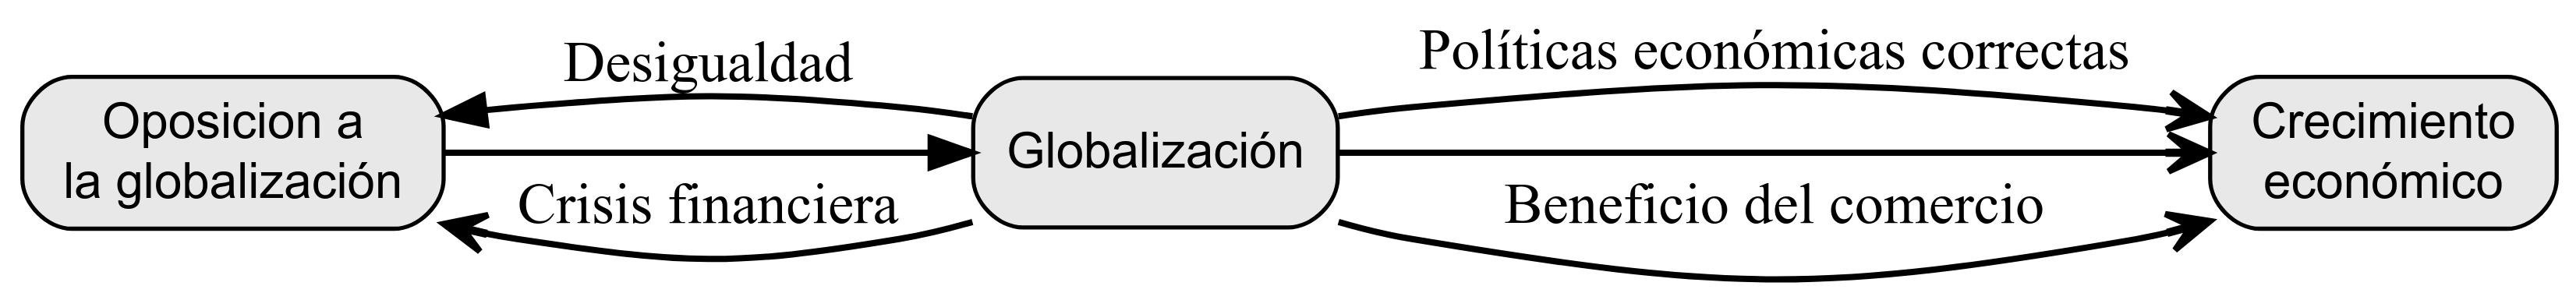
\includegraphics[width=5.5in,height=3.5in]{index_files/figure-latex/dot-figure-2.png}

}

\end{figure}

\hypertarget{cruxedticas-a-la-globalizaciuxf3n}{%
\subsection{Críticas a la
Globalización}\label{cruxedticas-a-la-globalizaciuxf3n}}

La globalización, a pesar de sus beneficios y oportunidades, también ha
sido objeto de críticas y preocupaciones por parte de diversos actores.
A continuación, se presentan algunas de las principales críticas a la
globalización:

\hypertarget{excesiva-volatilidad-de-los-precios}{%
\subsubsection{1. Excesiva volatilidad de los
precios}\label{excesiva-volatilidad-de-los-precios}}

La globalización ha llevado a una mayor interconexión de los mercados
internacionales, lo que puede resultar en una mayor volatilidad de los
precios de los bienes y servicios. Los cambios en la demanda y la oferta
a nivel global, así como los eventos económicos y políticos, pueden
tener un impacto significativo en los precios de los productos. Esta
volatilidad puede dificultar la planificación y la estabilidad económica
tanto a nivel microeconómico como macroeconómico.

\hypertarget{efecto-de-contagio}{%
\subsubsection{2. Efecto de contagio}\label{efecto-de-contagio}}

La interconexión de los mercados financieros y económicos a nivel global
puede llevar a un efecto de contagio, donde las crisis económicas o
financieras en un país se propagan rápidamente a otros países. Esto se
debe a la interdependencia de las economías y a la rápida transmisión de
información y capitales a través de las fronteras. El efecto de contagio
puede amplificar las crisis y dificultar su contención.

\hypertarget{tendencia-hacia-la-deflaciuxf3n}{%
\subsubsection{3. Tendencia hacia la
deflación}\label{tendencia-hacia-la-deflaciuxf3n}}

Algunos críticos argumentan que la globalización ha llevado a una
tendencia hacia la deflación, es decir, una disminución generalizada y
persistente de los precios. Esto se debe a la competencia global y la
presión sobre los costos de producción, lo que puede llevar a una
reducción de los precios de los bienes y servicios. La deflación puede
tener efectos negativos en la economía, como la disminución de los
ingresos y la demanda agregada.

\hypertarget{incremento-de-la-desigualdad-distributiva}{%
\subsubsection{4. Incremento de la desigualdad
distributiva}\label{incremento-de-la-desigualdad-distributiva}}

Se argumenta que la globalización ha contribuido al aumento de la
desigualdad distributiva en muchos países. A medida que las empresas se
expanden internacionalmente, tienden a buscar la maximización de sus
beneficios, lo que puede conducir a la explotación de la mano de obra
barata en países en desarrollo. Además, los beneficios de la
globalización pueden no distribuirse equitativamente, lo que resulta en
una mayor concentración de riqueza en manos de unos pocos, mientras que
otros experimentan un estancamiento o disminución de sus ingresos.

\hypertarget{tensiuxf3n-de-conflictos-por-limitados-mercados-y-recursos}{%
\subsubsection{5. Tensión de conflictos por limitados mercados y
recursos}\label{tensiuxf3n-de-conflictos-por-limitados-mercados-y-recursos}}

La globalización también ha generado tensiones y conflictos relacionados
con la competencia por mercados y recursos limitados. A medida que las
empresas buscan expandirse y obtener ventajas competitivas, pueden
surgir conflictos entre países por el acceso a recursos naturales, como
petróleo, minerales o agua. Estos conflictos pueden tener implicaciones
políticas, económicas y sociales.

\hypertarget{impacto-negativo-en-los-trabajadores-de-pauxedses-desarrollados}{%
\subsubsection{6. Impacto negativo en los trabajadores de países
desarrollados}\label{impacto-negativo-en-los-trabajadores-de-pauxedses-desarrollados}}

Una crítica común es que la globalización perjudica a los trabajadores
en los países desarrollados, ya que las empresas trasladan la producción
a países con mano de obra más barata. Esto puede resultar en la pérdida
de empleos en los países desarrollados y en una disminución de los
salarios. Los trabajadores pueden enfrentar dificultades para competir
en un mercado

laboral globalizado y pueden experimentar una mayor inseguridad laboral.

\hypertarget{reducciuxf3n-de-la-soberanuxeda-nacional}{%
\subsubsection{7. Reducción de la soberanía
nacional}\label{reducciuxf3n-de-la-soberanuxeda-nacional}}

La globalización plantea desafíos para la soberanía nacional, ya que
implica una mayor interdependencia y la necesidad de coordinación y
cooperación entre los países. Al participar en acuerdos comerciales y
organizaciones internacionales, los países pueden enfrentar limitaciones
a su autonomía para tomar decisiones económicas y políticas. Algunos
críticos argumentan que esto puede socavar la capacidad de los gobiernos
para proteger los intereses nacionales y satisfacer las necesidades de
sus ciudadanos.

\hypertarget{crisis-financieras-cada-vez-muxe1s-graves}{%
\subsubsection{8. Crisis financieras cada vez más
graves}\label{crisis-financieras-cada-vez-muxe1s-graves}}

Otra crítica importante es que la globalización ha llevado a una mayor
frecuencia y gravedad de las crisis financieras. La interconexión de los
mercados financieros internacionales ha aumentado la rapidez con la que
las crisis se propagan y puede dificultar la implementación de medidas
efectivas para controlarlas. Los flujos de capital especulativos y la
falta de regulación adecuada pueden contribuir a la aparición de crisis
financieras sistémicas.


\printbibliography


\end{document}
